% ============================================================
%  鱼你有图 概要设计说明书
%  编译方式: xelatex main.tex
%  文档类: ctexart (中文文章)
% ============================================================
\documentclass[12pt,a4paper]{ctexart}

% ---------- 页面设置 ----------
\usepackage[top=2.5cm,bottom=2.5cm,left=2.8cm,right=2.8cm]{geometry}

% ---------- 字体 ----------
\usepackage{fontspec}

% ---------- 图表 ----------
\usepackage{graphicx}
\usepackage{float}
\usepackage{subcaption}
\graphicspath{{figures/}}

% ---------- 表格 ----------
\usepackage{tabularx}
\usepackage{longtable}
\usepackage{booktabs}
\usepackage{array}
\usepackage{multirow}

% ---------- 代码块 ----------
\usepackage{listings}
\usepackage{xcolor}

\definecolor{codebg}{RGB}{248,248,248}
\definecolor{codeframe}{RGB}{220,220,220}
\definecolor{codekey}{RGB}{0,119,170}
\definecolor{codestr}{RGB}{17,140,55}
\definecolor{codecmt}{RGB}{138,138,138}

\lstset{
  basicstyle          = \small\ttfamily,
  backgroundcolor     = \color{codebg},
  frame               = single,
  framerule           = 0.5pt,
  rulecolor           = \color{codeframe},
  numbers             = left,
  numberstyle         = \tiny\color{gray},
  numbersep           = 6pt,
  breaklines          = true,
  breakatwhitespace   = false,
  showstringspaces    = false,
  captionpos          = t,
  aboveskip           = 8pt,
  belowskip           = 8pt,
  keywordstyle        = \color{codekey}\bfseries,
  stringstyle         = \color{codestr},
  commentstyle        = \color{codecmt}\itshape,
  extendedchars       = true,
  literate            =
    {。}{{。}}1
    {，}{{，}}1
    {；}{{；}}1
    {：}{{：}}1
    {！}{{！}}1
    {？}{{？}}1
    {（}{{（}}1
    {）}{{）}}1
    {「}{{「}}1
    {」}{{」}}1
}

% ---------- 超链接 ----------
\usepackage[colorlinks=true,linkcolor=blue,urlcolor=blue,citecolor=blue]{hyperref}

% ---------- 页眉页脚 ----------
\usepackage{fancyhdr}
\pagestyle{fancy}
\fancyhf{}
\fancyhead[L]{\small 鱼你有图概要设计说明书}
\fancyhead[R]{\small 专业综合实习}
\fancyfoot[C]{\thepage}
\renewcommand{\headrulewidth}{0.5pt}

% ---------- 标题格式 ----------
\ctexset{
  section = {
    format    = \Large\bfseries,
    number    = \thesection,
    aftername = \quad,
  },
  subsection = {
    format    = \large\bfseries,
    number    = \thesubsection,
    aftername = \quad,
  },
}

% ---------- 文档标题 ----------
\title{\Huge\bfseries 鱼你有图概要设计说明书}
\author{}
\date{}

\begin{document}

% ===== 封面 =====
\begin{titlepage}
  \centering
  \vspace*{3cm}

  {\Huge\bfseries 鱼你有图概要设计说明书\par}
  \vspace{0.8cm}
  {\LARGE 面向垂钓场景的 GIS 智能推荐与社交平台\par}

  \vspace{2.5cm}

  \begin{tabular}{rl}
    \textbf{项目类型} & 专业综合实习课程项目 \\[6pt]
    \textbf{版本号}   & v1.0 \\[6pt]
    \textbf{编写日期} & \today \\
  \end{tabular}

  \vspace{2cm}
  {\large 武汉大学}
\end{titlepage}

% ===== 目录 =====
\tableofcontents
\newpage

% ============================================================
%  第1章 文档说明
% ============================================================
\section{文档说明}

\subsection{编写目的}

本文档是“鱼你有图”项目的概要设计说明书，旨在基于已通过评审的需求分析文档与原型成果，回答“系统应当如何实现”这一核心问题。文档面向开发团队、测试人员及项目管理人员，作为详细设计与编码阶段的纲领性依据。

本文档的预期读者包括：
\begin{itemize}
  \item \textbf{开发人员}：理解系统总体结构、模块划分与接口约定，指导编码实现；
  \item \textbf{测试人员}：依据模块职责与接口定义，设计集成测试与系统测试用例；
  \item \textbf{项目管理人员}：把握系统边界、技术选型与部署方案，进行进度与风险管理。
\end{itemize}

\subsection{文档范围}

本文档覆盖以下设计内容：
\begin{enumerate}
  \item 系统总体架构设计，包括前后端分层结构与模块组织方式；
  \item 技术架构选型，包括前端框架、后端框架、数据持久化方案及外部服务集成；
  \item 系统部署方案，包括开发环境与生产环境的拓扑结构；
  \item 外部系统接口设计，包括高德地图 API 与 DeepSeek AI 服务的集成方式；
  \item 系统模块划分与模块间调用关系；
  \item 核心视图设计，包括用例视图、逻辑视图、数据视图、组件视图与并发视图；
  \item 数据持久化设计，包括数据集合的概念结构与逻辑结构；
  \item RESTful API 接口设计与并发控制策略；
  \item 通用子系统设计，包括位置隐私保护、错误处理与配置管理等机制。
\end{enumerate}

本文档不包含以下内容：前端页面控件的详细布局与样式定义、函数级实现细节、具体代码逻辑、数据库 SQL 语句（系统采用 JSON 文件存储）。

\subsection{术语与缩写}

\begin{table}[H]
  \centering
  \caption{术语与缩写说明}
  \label{tab:glossary}
  \begin{tabular}{p{3cm}p{9cm}}
    \toprule
    \textbf{术语/缩写} & \textbf{说明} \\
    \midrule
    POI & Point of Interest，兴趣点，本系统中指钓点 \\
    GIS & Geographic Information System，地理信息系统 \\
    AMap & 高德地图，提供 JS API（前端地图渲染）与 Web Service API（后端 POI 搜索、天气查询） \\
    DeepSeek & 大语言模型服务，用于生成自然语言出钓建议 \\
    RESTful API & 遵循 REST 架构风格的 HTTP 接口 \\
    SPA & Single Page Application，单页面应用 \\
    JSON Store & 基于 JSON 文件的数据持久化方案，以文件系统模拟 NoSQL 数据库 \\
    CORS & Cross-Origin Resource Sharing，跨域资源共享 \\
    单级会员 & 系统中会员仅设 active/inactive/expired 三种状态，不区分等级 \\
    \bottomrule
  \end{tabular}
\end{table}

\subsection{参考文献}

\begin{enumerate}
  \item 《鱼你有图需求分析文档》
  \item 《鱼你有图项目功能差距与修改路线》（docs/创新产品设计/03\_差距分析与路线/）
  \item FastAPI 官方文档：\url{https://fastapi.tiangolo.com/}
  \item Vue 3 官方文档：\url{https://cn.vuejs.org/}
  \item 高德地图 JS API 文档：\url{https://lbs.amap.com/api/jsapi-v2/summary}
  \item 高德 Web 服务 API 文档：\url{https://lbs.amap.com/api/webservice/summary}
\end{enumerate}

\newpage

% ============================================================
%  第2章 系统背景
% ============================================================
\section{系统背景}

\subsection{项目概述}

“鱼你有图”是面向钓鱼爱好者的垂钓 GIS 社交平台。平台将地图找点、POI 详情、规则推荐、鱼获发布、社区展示和教程学习整合在同一链路中，帮助用户快速判断“去哪钓、能不能钓、现在适不适合钓”。

系统以高德地图为地理信息服务底座，以规则模型与 AI 大语言模型协同驱动智能推荐，以 JSON 文件存储实现轻量化数据持久化，以前后端分离架构保证开发效率与部署灵活性。

\subsection{系统目标}

\begin{enumerate}
  \item \textbf{钓点发现}：基于高德地图 POI 搜索与 Haversine 距离计算，帮助用户按城市、关键词、距离筛选钓点；
  \item \textbf{智能推荐}：综合鱼情、合规性、天气、距离、设施、社交热度六维评分，排序推荐最优钓点；
  \item \textbf{出钓记录}：完整记录每次出钓的鱼种、数量、重量、钓法、饵料等数据，支持数据分析与报告生成；
  \item \textbf{社区互动}：支持图文帖子发布、评论、点赞/收藏、关注/好友等社交功能，并内置位置隐私保护；
  \item \textbf{活动与群聊}：支持线下钓鱼活动的创建、报名、签到，以及群组即时通讯；
  \item \textbf{技能成长}：提供分级教程体系，记录用户学习进度，并结合出钓数据生成个性化服务推荐；
  \item \textbf{装备商城}：提供装备浏览与下单功能（Demo 阶段为模拟支付）。
\end{enumerate}

\subsection{系统范围}

\begin{table}[H]
  \centering
  \caption{系统功能范围}
  \label{tab:scope}
  \begin{tabular}{p{2.5cm}p{3cm}p{6.5cm}}
    \toprule
    \textbf{功能域} & \textbf{范围} & \textbf{说明} \\
    \midrule
    地图与钓点 & 包含 & POI 搜索、列表、详情、距离计算、高德地图渲染 \\
    智能推荐 & 包含 & 六维评分排序、天气集成、AI 自然语言建议 \\
    出钓记录 & 包含 & 记录 CRUD、鱼获明细、空军标记、装备关联 \\
    社区帖子 & 包含 & 图文帖发布/列表/详情、多维度筛选、信息流 \\
    社区互动 & 包含 & 评论、点赞/收藏、关注/好友、私信、通知 \\
    活动管理 & 包含 & 活动创建、报名、签到、活动记录自动生成 \\
    群组聊天 & 包含 & 群组列表、群消息发送/接收 \\
    用户与会员 & 包含 & 用户资料、单级会员状态 \\
    数据分析 & 包含 & 偏好/效率分离的个人档案与报告 \\
    教程学习 & 包含 & 教程列表、学习进度追踪 \\
    装备商城 & 包含（Demo） & 装备浏览、下单、模拟支付 \\
    用户认证 & 不包含（当前） & 当前采用 demo\_user 硬编码，认证体系待后续实现 \\
    图像上传 & 不包含（当前） & 图片以 URL 字符串存储，未实现文件上传服务 \\
    移动端适配 & 不包含（当前） & 当前仅适配桌面浏览器 \\
    \bottomrule
  \end{tabular}
\end{table}

\subsection{用户角色}

\begin{table}[H]
  \centering
  \caption{用户角色定义}
  \label{tab:roles}
  \begin{tabular}{p{2.5cm}p{4cm}p{5.5cm}}
    \toprule
    \textbf{角色} & \textbf{特征} & \textbf{核心需求} \\
    \midrule
    普通用户（非会员） & 未开通会员 & 使用社区、记录、教程基础功能；报告能力受限 \\
    会员用户 & 会员状态为 active & 完整个人档案、报告生成与分享、个性化推荐 \\
    管理员 & 系统运营者 & 管理 POI 数据、教程内容、社区内容审核（当前 Demo 未实现管理后台） \\
    \bottomrule
  \end{tabular}
\end{table}

\newpage

% ============================================================
%  第3章 总体架构设计
% ============================================================
\section{总体架构设计}

\subsection{系统架构视图}

系统采用前后端分离的 B/S 架构，前端为基于 Vue 3 的单页面应用（SPA），后端为基于 FastAPI 的 RESTful API 服务，数据层采用 JSON 文件集合模拟 NoSQL 数据库。前端通过 Vite 开发服务器的代理机制将 /api 请求转发至后端，生产环境可部署至同一域名或通过反向代理统一入口。

\begin{figure}[H]
  \centering
  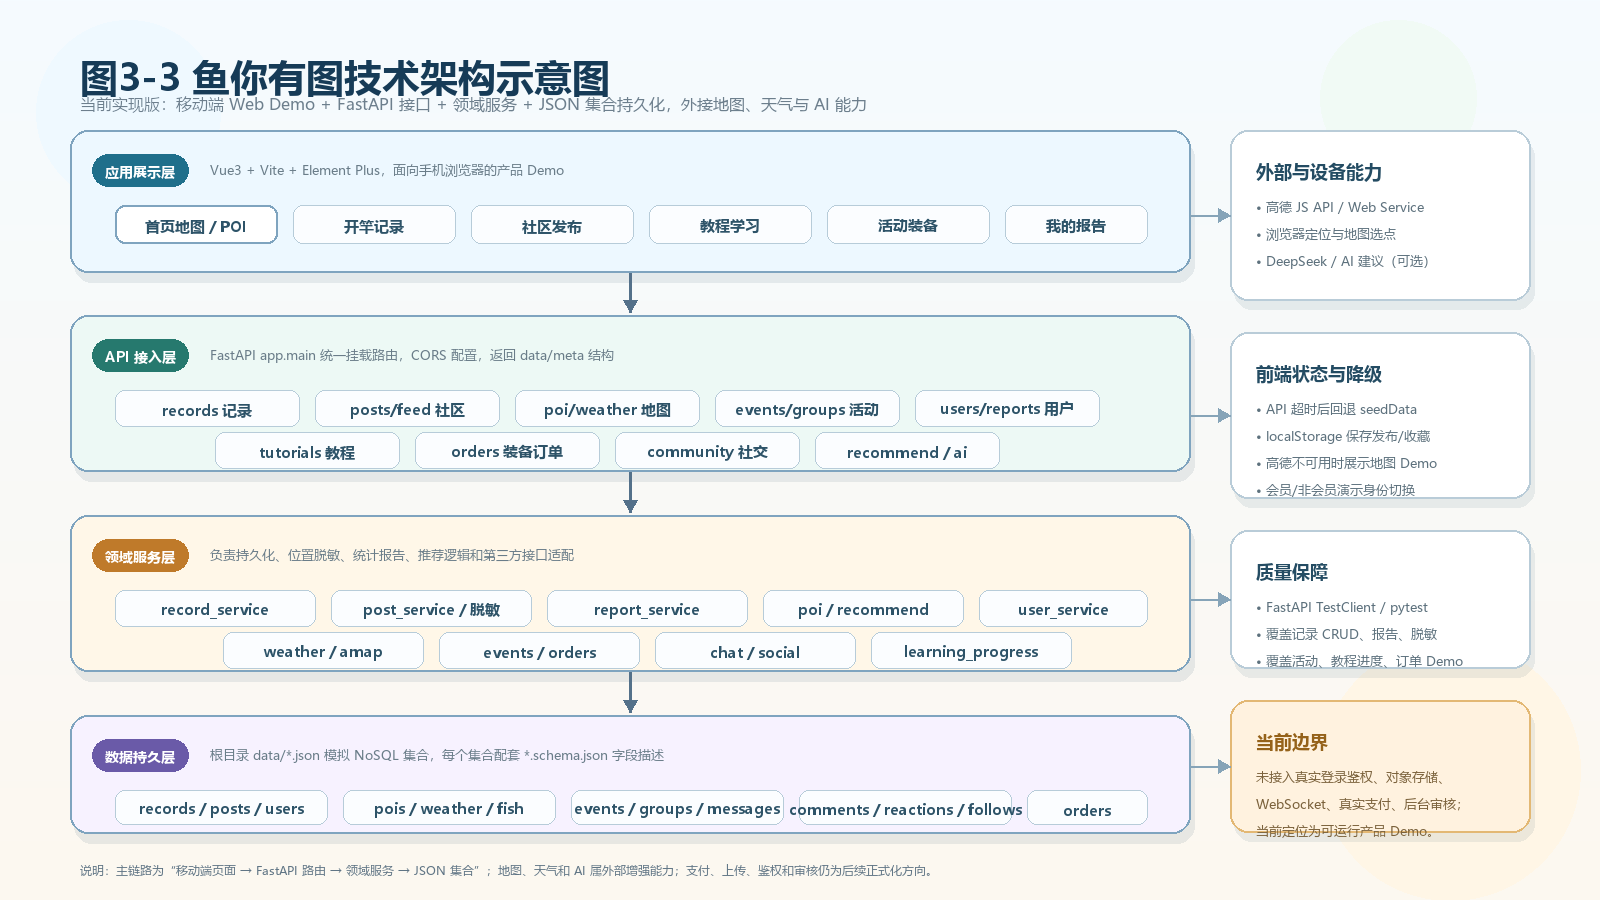
\includegraphics[width=0.95\textwidth]{figures/yuni-architecture.png}
  \caption{系统总体架构图}
  \label{fig:architecture}
\end{figure}

\subsection{分层架构}

系统自上而下分为四层：

\begin{enumerate}
  \item \textbf{表示层（Presentation Layer）}：Vue 3 + Vite + Element Plus，负责页面渲染、用户交互、地图展示（高德 JS API）。前端通过 Tab 切换视图，无 vue-router，所有 API 调用集中于 \texttt{frontend/src/services/api.js}。

  \item \textbf{接口层（API Layer）}：FastAPI 路由层，位于 \texttt{backend/app/api/}，包含 14 个路由模块。负责 HTTP 请求解析、参数校验（Pydantic 模型）、响应序列化。路由层不包含业务逻辑，仅调用服务层并返回统一格式的 JSON 响应。

  \item \textbf{服务层（Service Layer）}：位于 \texttt{backend/app/services/}，包含 11 个服务模块。负责业务逻辑实现，包括推荐算法、报告计算、位置脱敏、AI 建议生成等。服务层通过数据层访问持久化数据，通过 httpx 调用外部 API。

  \item \textbf{数据层（Data Layer）}：位于 \texttt{backend/app/data/json\_store.py}，提供 \texttt{load\_collection}、\texttt{save\_collection}、\texttt{update\_collection} 三个核心函数。写入采用临时文件 + 原子替换策略，保证数据一致性。所有数据存储在根目录 \texttt{data/} 下的 JSON 文件中。
\end{enumerate}

\begin{figure}[H]
  \centering
  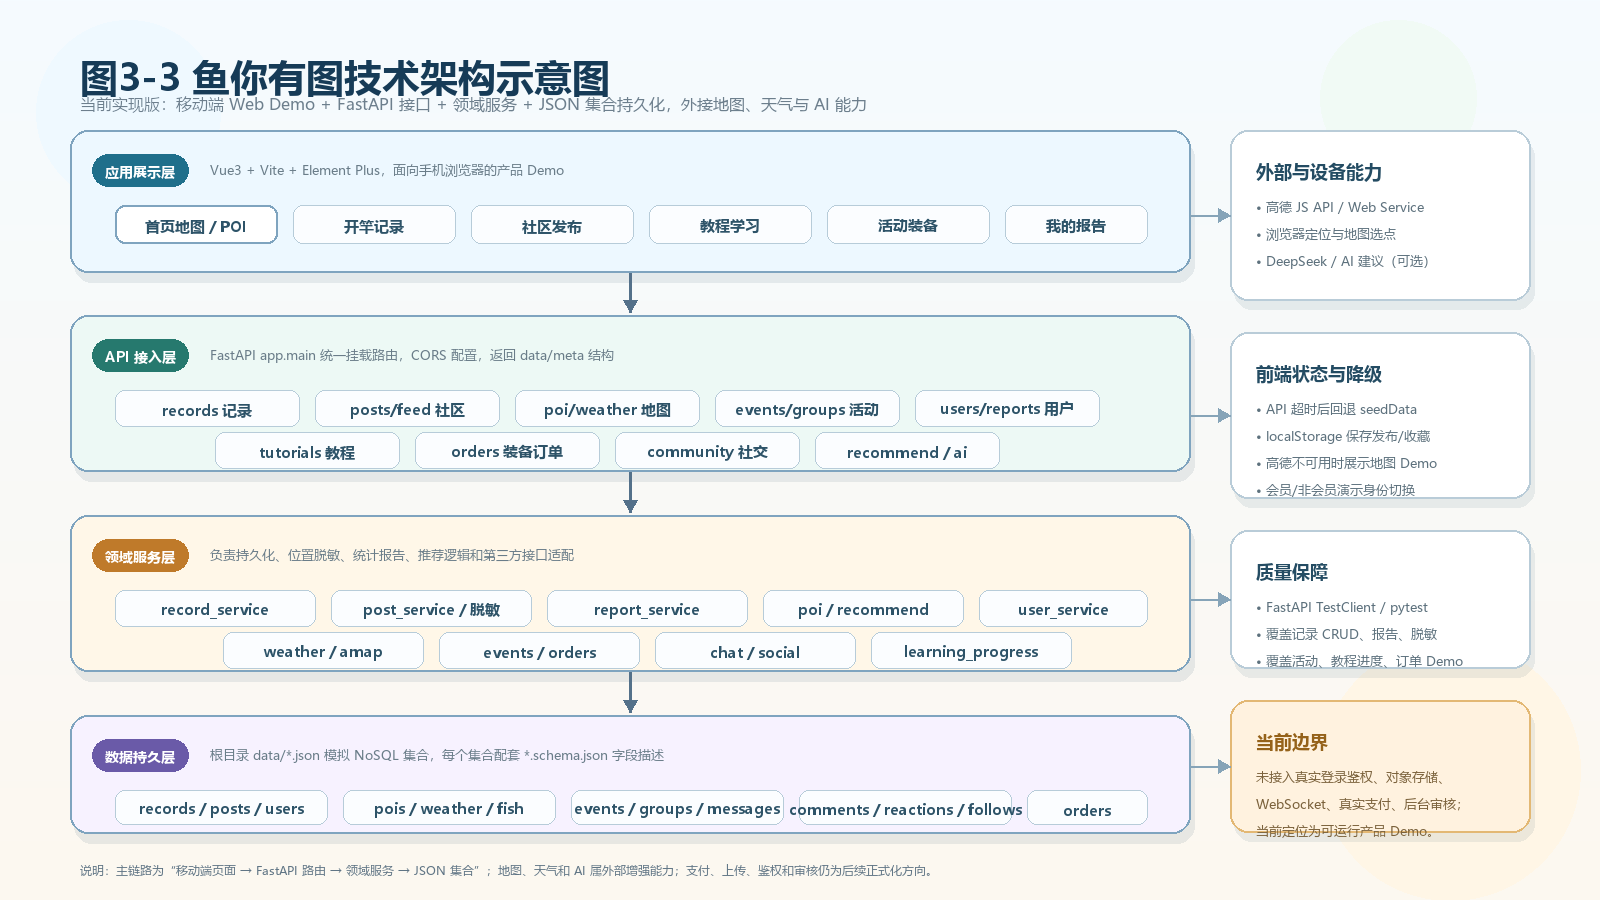
\includegraphics[width=0.9\textwidth]{figures/tech-architecture.png}
  \caption{系统分层架构与技术栈}
  \label{fig:layered-arch}
\end{figure}

\subsection{前端架构}

前端为无路由的单页面应用（SPA），\texttt{App.vue} 通过响应式变量 \texttt{currentTab} 切换视图组件。共包含 14 个视图组件，按功能域组织：

\begin{table}[H]
  \centering
  \caption{前端视图组件一览}
  \label{tab:frontend-components}
  \begin{tabular}{p{3cm}p{3cm}p{6cm}}
    \toprule
    \textbf{组件} & \textbf{所属 Tab} & \textbf{功能说明} \\
    \midrule
    HomeView.vue & 首页 & 地图面板、POI 卡片、推荐入口 \\
    MapPanel.vue & 首页（子组件） & 高德地图渲染、POI 标记交互 \\
    PoiCard.vue & 首页（子组件） & POI 详情卡片展示 \\
    CommunityView.vue & 社区 & 帖子信息流、多维度筛选 \\
    PostViewer.vue & 社区（子组件） & 帖子详情与评论查看 \\
    PublishView.vue & 社区（子组件） & 帖子发布表单 \\
    RecordView.vue & 记录 & 出钓记录列表与详情 \\
    RecordLocationDialog.vue & 记录（子组件） & 钓点位置选择对话框 \\
    TutorialsView.vue & 技巧 & 教程列表与学习进度 \\
    ServicesView.vue & 服务 & 个人报告、会员、装备推荐 \\
    MineView.vue & 我的 & 个人中心入口 \\
    UserProfileView.vue & 我的（子组件） & 用户资料展示 \\
    ChatView.vue & 社区 & 群聊与私信界面 \\
    FishingView.vue & 记录 & 鱼获数据录入表单 \\
    \bottomrule
  \end{tabular}
\end{table}

Vite 开发服务器配置了代理规则：所有 \texttt{/api} 前缀的请求转发至 \texttt{http://127.0.0.1:8000}。生产构建时通过环境变量 \texttt{VITE\_API\_BASE\_URL} 指定后端地址。前端 API 调用层实现了统一的超时控制（1800ms）和错误回退机制，后端不可用时回退到内置种子数据（seedData）。

\subsection{后端架构}

后端基于 FastAPI 框架，入口文件为 \texttt{backend/app/main.py}。应用创建时配置 CORS 中间件，允许前端开发服务器跨域访问。14 个路由模块通过 \texttt{app.include\_router} 注册，统一挂载在 \texttt{/api} 前缀下。

\begin{table}[H]
  \centering
  \caption{后端路由模块一览}
  \label{tab:backend-routes}
  \begin{tabular}{p{3.5cm}p{2.5cm}p{6cm}}
    \toprule
    \textbf{路由模块} & \textbf{前缀} & \textbf{主要端点} \\
    \midrule
    routes\_meta & /api & /health, /amap/config \\
    routes\_records & /api & /records CRUD \\
    routes\_posts & /api & /posts, /feed \\
    routes\_users & /api & /users/\{id\}, /users/\{id\}/membership \\
    routes\_community & /api & /posts/\{id\}/comments, /posts/\{id\}/reactions, /users/\{id\}/follow, /users/\{id\}/social, /users/\{id\}/friend, /direct-messages, /users/\{id\}/notifications \\
    routes\_events & /api & /events CRUD, /events/\{id\}/register, /events/\{id\}/checkin, /groups, /equipment \\
    routes\_reports & /api & /users/\{id\}/profile-summary, /users/\{id\}/reports, /users/\{id\}/service-recommendations \\
    routes\_recommend & /api & /recommendations \\
    routes\_ai & /api & /ai/fishing-advice \\
    routes\_weather & /api & /weather/current \\
    routes\_poi & /api & /pois, /pois/\{id\} \\
    routes\_tutorials & /api & /tutorials, /users/\{id\}/learning-progress \\
    routes\_orders & /api & /users/\{id\}/orders, /orders, /orders/\{id\}/pay \\
    routes\_fish & /api & /fish-species/\{name\} \\
    \bottomrule
  \end{tabular}
\end{table}

\subsection{数据架构}

系统采用基于 JSON 文件的内存缓存 + 原子写入的持久化方案。数据层在模块加载时将 JSON 文件读入内存列表，业务操作直接操作内存数据，写操作通过 \texttt{save\_collection} 以临时文件 + 原子替换的方式写回磁盘。该方案在单用户 Demo 场景下兼顾了开发效率与数据可靠性。

\newpage

% ============================================================
%  第4章 技术架构设计
% ============================================================
\section{技术架构设计}

\subsection{技术选型总览}

\begin{table}[H]
  \centering
  \caption{技术选型一览}
  \label{tab:tech-stack}
  \begin{tabular}{p{3cm}p{3cm}p{6cm}}
    \toprule
    \textbf{层次} & \textbf{技术} & \textbf{版本/说明} \\
    \midrule
    前端框架 & Vue 3 & Composition API + \texttt{<script setup>} \\
    构建工具 & Vite 5 & 开发服务器热重载，代理转发 \\
    UI 组件库 & Element Plus & 2.14.x，提供表单、卡片、对话框等组件 \\
    地图 SDK & 高德 JS API 2.0 & 前端地图渲染、POI 标记 \\
    后端框架 & FastAPI & 0.115.x，异步支持 \\
    数据校验 & Pydantic 2 & 请求/响应模型定义与序列化 \\
    配置管理 & pydantic-settings & 从 .env 文件读取配置 \\
    HTTP 客户端 & httpx & 0.27.x，异步调用外部 API \\
    服务器 & Uvicorn & ASGI 服务器，支持热重载 \\
    数据存储 & JSON 文件 & 23 个集合，每集合配 .schema.json \\
    外部 API & 高德 Web 服务 API & POI 搜索、天气查询 \\
    AI 服务 & DeepSeek API & deepseek-chat 模型，出钓建议生成 \\
    环境管理 & conda & fish 环境 \\
    开发语言 & Python 3.x + JavaScript (ES Module) & — \\
    \bottomrule
  \end{tabular}
\end{table}

\subsection{前端技术详述}

\subsubsection{Vue 3 Composition API}

前端统一使用 Composition API 的 \texttt{<script setup>} 语法。状态管理采用 reactive/ref 响应式变量，未引入 Vuex/Pinia 等全局状态管理库。跨组件数据共享通过 props 传递与 localStorage 读写实现。

\subsubsection{高德 JS API 集成}

地图组件 \texttt{MapPanel.vue} 通过异步加载高德 JS API 2.0 SDK。前端在应用启动时调用 \texttt{/api/amap/config} 获取 JS API Key 与安全码，动态注入地图脚本。地图功能包括：POI 标记展示、当前位置定位、点击 POI 查看详情。

\subsubsection{API 调用层}

前端所有 HTTP 请求统一封装在 \texttt{api.js} 中，特点包括：
\begin{itemize}
  \item 统一超时控制：每个请求 1800ms 超时，通过 AbortController 实现；
  \item 错误回退：后端不可用时回退到内置 seedData，保证 Demo 体验不中断；
  \item 离线标记：创建操作失败时返回带 \texttt{offline: true} 标记的本地对象；
  \item URL 解析：支持通过 \texttt{VITE\_API\_BASE\_URL} 环境变量指定后端地址。
\end{itemize}

\subsection{后端技术详述}

\subsubsection{FastAPI 应用结构}

FastAPI 应用在 \texttt{main.py} 中创建，配置了：
\begin{itemize}
  \item CORS 中间件：允许 \texttt{localhost:5173} 和 \texttt{127.0.0.1:5173} 的跨域请求；
  \item 路由注册：14 个路由模块统一挂载在 \texttt{/api} 前缀；
  \item 应用元信息：标题“鱼你有图”，版本号 0.3.0。
\end{itemize}

\subsubsection{配置管理}

配置类 \texttt{Settings} 继承 \texttt{pydantic\_settings.BaseSettings}，从根目录 \texttt{.env} 文件读取环境变量。通过 \texttt{@lru\_cache} 装饰器实现单例模式。主要配置项包括：

\begin{table}[H]
  \centering
  \caption{系统配置项}
  \label{tab:config}
  \begin{tabular}{p{4.5cm}p{7.5cm}}
    \toprule
    \textbf{配置项} & \textbf{说明} \\
    \midrule
    AMAP\_WEB\_SERVICE\_KEY & 高德 Web 服务 API Key，后端 POI 搜索与天气查询 \\
    AMAP\_JS\_API\_KEY & 高德 JS API Key，前端地图渲染 \\
    AMAP\_SECURITY\_CODE & 高德 JS API 安全码 \\
    DEEPSEEK\_API\_KEY & DeepSeek API 密钥 \\
    DEEPSEEK\_BASE\_URL & DeepSeek API 地址，默认 https://api.deepseek.com \\
    DEEPSEEK\_MODEL & 模型名称，默认 deepseek-chat \\
    APP\_ENV & 运行环境，development 或 production \\
    FRONTEND\_ORIGIN & 前端开发服务器地址，CORS 白名单 \\
    DEFAULT\_CITY\_CODE & 默认城市编码，默认 420100（武汉市） \\
    \bottomrule
  \end{tabular}
\end{table}

\subsubsection{Pydantic 数据模型}

系统使用 Pydantic 2 定义请求与响应模型，位于 \texttt{backend/app/schemas/}。模型按业务域组织：
\begin{itemize}
  \item \texttt{record.py}：FishingRecordCreate、FishingRecordPatch、FishingRecord 等；
  \item \texttt{post.py}：CatchPostCreate、CatchPost 等；
  \item \texttt{user.py}：User、Membership；
  \item \texttt{poi.py}：FishingPOI，包含 30+ 字段；
  \item \texttt{recommendation.py}：RecommendationRequest、RecommendationItem 等；
  \item \texttt{event.py}：EventCreate、GroupMessageCreate、UserAction；
  \item \texttt{weather.py}：WeatherSnapshot；
  \item \texttt{order.py}：OrderCreate、OrderAction；
  \item \texttt{tutorial.py}：LearningProgressUpdate。
\end{itemize}

所有响应模型遵循统一格式：\texttt{\{"data": ...\}} 或 \texttt{\{"data": ..., "meta": ...\}}。

\subsection{数据存储技术}

系统采用 JSON 文件集合模拟 NoSQL 数据库，未使用关系型数据库或 ORM。数据层核心特点：

\begin{itemize}
  \item \textbf{原子写入}：通过 \texttt{tempfile.mkstemp} 创建临时文件，写入完成后 \texttt{os.replace} 原子替换目标文件；
  \item \textbf{深拷贝隔离}：\texttt{load\_collection} 返回 \texttt{deepcopy}，避免业务层意外修改缓存；
  \item \textbf{集合 Schema 约束}：每个 \texttt{.json} 数据文件配有同名 \texttt{.schema.json} 描述文件，规范字段定义；
  \item \textbf{模块级缓存}：\texttt{record\_service} 和 \texttt{post\_service} 在模块加载时将集合加载为模块变量，后续读写直接操作内存，仅在写操作时持久化。
\end{itemize}

\newpage

% ============================================================
%  第5章 部署设计
% ============================================================
\section{部署设计}

\subsection{部署拓扑}

系统部署分为开发环境与生产环境两种模式。

\subsubsection{开发环境}

开发环境采用前后端分离部署，分别运行于不同端口：

\begin{figure}[H]
  \centering
  % 部署拓扑图（暂缺，保留图位）
  \fbox{\parbox{0.8\textwidth}{\centering\vspace{3cm}部署拓扑示意图（待补充）\vspace{3cm}}}
  \caption{开发环境部署拓扑}
  \label{fig:deploy-topology}
\end{figure}

\begin{itemize}
  \item \textbf{前端开发服务器}：Vite Dev Server，监听 0.0.0.0:5173，通过代理将 /api 请求转发至后端；
  \item \textbf{后端 API 服务器}：Uvicorn，监听 127.0.0.1:8000，支持 --reload 热重载；
  \item \textbf{数据存储}：本地文件系统，\texttt{data/} 目录下的 JSON 文件；
  \item \textbf{外部服务}：通过公网访问高德 API 与 DeepSeek API。
\end{itemize}

启动命令如下：

\begin{lstlisting}[caption={开发环境启动命令},label={lst:startup}]
# 后端
conda activate fish
cd backend
uvicorn app.main:app --reload --host 127.0.0.1 --port 8000

# 前端
cd frontend
npm run dev    # http://localhost:5173
\end{lstlisting}

\subsubsection{生产环境}

生产环境建议方案：
\begin{itemize}
  \item 前端构建为静态资源（\texttt{npm run build}），部署至 Nginx 或 CDN；
  \item 后端通过 Uvicorn 多 worker 模式运行，前置 Nginx 反向代理；
  \item 环境变量 \texttt{APP\_ENV=production}，启用 DeepSeek AI 与高德 Web 服务 API 的远程调用；
  \item JSON 数据文件部署于服务器本地磁盘或挂载卷，定期备份。
\end{itemize}

\subsection{运行环境要求}

\begin{table}[H]
  \centering
  \caption{运行环境要求}
  \label{tab:env-req}
  \begin{tabular}{p{3cm}p{4cm}p{5cm}}
    \toprule
    \textbf{组件} & \textbf{最低要求} & \textbf{推荐配置} \\
    \midrule
    操作系统 & macOS / Linux / Windows & Ubuntu 20.04+ / macOS 12+ \\
    Python & 3.10+ & 3.11+ \\
    Node.js & 18.x & 20.x LTS \\
    conda & 任意版本 & 24.x \\
    磁盘空间 & 100 MB & 500 MB+ \\
    内存 & 512 MB & 2 GB+ \\
    \bottomrule
  \end{tabular}
\end{table}

\newpage

% ============================================================
%  第6章 外部接口设计
% ============================================================
\section{外部接口设计}

\subsection{外部系统接口总览}

系统依赖两个外部服务：高德地图开放平台和 DeepSeek AI 平台。

\begin{table}[H]
  \centering
  \caption{外部系统接口一览}
  \label{tab:external-apis}
  \begin{tabular}{p{2.5cm}p{2.5cm}p{3cm}p{4cm}}
    \toprule
    \textbf{外部系统} & \textbf{接口} & \textbf{调用方} & \textbf{用途} \\
    \midrule
    高德 JS API & AMap.Map 等 & 前端 & 地图渲染、POI 标记 \\
    高德 Web 服务 & /v5/place/text & 后端 & POI 关键词搜索 \\
    高德 Web 服务 & /v5/place/around & 后端 & 周边 POI 搜索 \\
    高德 Web 服务 & /v3/weather/weatherInfo & 后端 & 实时天气查询 \\
    DeepSeek & /chat/completions & 后端 & AI 出钓建议生成 \\
    \bottomrule
  \end{tabular}
\end{table}

\subsection{高德 JS API 接口}

前端通过异步脚本加载高德 JS API 2.0，加载 URL 格式为：

\begin{lstlisting}[caption={高德 JS API 加载方式},label={lst:amap-js}]
https://webapi.amap.com/maps?v=2.0&key={JS_API_KEY}&security={SECURITY_CODE}
\end{lstlisting}

前端在应用初始化时调用 \texttt{/api/amap/config} 获取 key 和 securityCode，动态创建 script 标签注入页面。主要使用的 JS API 包括：
\begin{itemize}
  \item \texttt{AMap.Map}：创建地图实例；
  \item \texttt{AMap.Marker}：POI 点位标记；
  \item \texttt{AMap.InfoWindow}：POI 信息弹窗；
  \item \texttt{AMap.Geolocation}：用户定位。
\end{itemize}

\subsection{高德 Web 服务 API 接口}

\subsubsection{POI 搜索接口}

后端 \texttt{amap\_service.py} 封装了两个搜索模式：

\textbf{文本搜索}（\texttt{/v5/place/text}）：
\begin{table}[H]
  \centering
  \caption{高德 POI 文本搜索参数}
  \label{tab:amap-text-search}
  \begin{tabular}{p{2.5cm}p{2cm}p{7.5cm}}
    \toprule
    \textbf{参数} & \textbf{必填} & \textbf{说明} \\
    \midrule
    key & 是 & Web 服务 API Key \\
    keywords & 是 & 搜索关键词，如“钓场”“野钓” \\
    city & 否 & 城市名称或编码，限定搜索范围 \\
    output & 否 & 输出格式，固定 JSON \\
    page\_size & 否 & 每页条数，默认 10 \\
    \bottomrule
  \end{tabular}
\end{table}

\textbf{周边搜索}（\texttt{/v5/place/around}）：
\begin{table}[H]
  \centering
  \caption{高德 POI 周边搜索参数}
  \label{tab:amap-around-search}
  \begin{tabular}{p{2.5cm}p{2cm}p{7.5cm}}
    \toprule
    \textbf{参数} & \textbf{必填} & \textbf{说明} \\
    \midrule
    key & 是 & Web 服务 API Key \\
    location & 是 & 中心点坐标，格式 "lng,lat" \\
    keywords & 否 & 搜索关键词 \\
    radius & 否 & 搜索半径，单位米，默认 8000 \\
    \bottomrule
  \end{tabular}
\end{table}

\subsubsection{天气查询接口}

\begin{lstlisting}[caption={高德天气 API 调用方式},label={lst:amap-weather}]
GET https://restapi.amap.com/v3/weather/weatherInfo
  ?key={KEY}&city={adcode}&extensions=base&output=JSON
\end{lstlisting}

天气服务仅在 \texttt{APP\_ENV=production} 且配置了 API Key 时调用高德接口，开发环境使用种子天气数据。响应字段包括：weather（天气现象）、temperature（气温）、winddirection（风向）、windpower（风力）、humidity（湿度）。

\subsection{DeepSeek AI 接口}

后端 \texttt{ai\_service.py} 封装了 DeepSeek 的 Chat Completions API 调用：

\begin{lstlisting}[caption={DeepSeek API 调用方式},label={lst:deepseek}]
POST https://api.deepseek.com/chat/completions
Authorization: Bearer {DEEPSEEK_API_KEY}
Content-Type: application/json

{
  "model": "deepseek-chat",
  "messages": [
    {"role": "system", "content": "你是鱼你有图项目的出钓建议解释器..."},
    {"role": "user", "content": "..."}
  ],
  "temperature": 0.2
}
\end{lstlisting}

调用策略：
\begin{itemize}
  \item 仅在 \texttt{APP\_ENV=production} 且配置了 \texttt{DEEPSEEK\_API\_KEY} 时调用远程 API；
  \item development 环境下返回基于规则模型的 Mock 建议；
  \item 远程调用超时时间为 20 秒；
  \item 调用失败时静默回退到 Mock 建议，不影响前端体验。
\end{itemize}

AI 服务定位为“解释器”而非“决策器”：推荐排序由规则模型完成，AI 仅负责将排序结果转化为自然语言解释和建议。

\subsection{接口协议与数据格式}

所有外部接口均采用 HTTPS 协议，请求与响应格式为 JSON。后端使用 httpx 的 \texttt{AsyncClient} 进行异步调用，设置合理的超时时间以避免阻塞主线程。

\newpage

% ============================================================
%  第7章 模块划分
% ============================================================
\section{模块划分}

\subsection{模块命名规范}

系统模块按功能域划分为 11 个一级模块，每个模块由前端视图组件与后端路由/服务层协同构成。

\begin{table}[H]
  \centering
  \caption{系统模块命名表}
  \label{tab:module-names}
  \begin{tabular}{p{1.5cm}p{2.5cm}p{4cm}p{4cm}}
    \toprule
    \textbf{编号} & \textbf{模块名称} & \textbf{前端组件} & \textbf{后端路由/服务} \\
    \midrule
    M01 & 地图钓点 & HomeView, MapPanel, PoiCard & routes\_poi, poi\_service, amap\_service \\
    M02 & 智能推荐 & HomeView（推荐面板） & routes\_recommend, recommend\_service \\
    M03 & 出钓记录 & RecordView, FishingView, RecordLocationDialog & routes\_records, record\_service \\
    M04 & 社区帖子 & CommunityView, PublishView, PostViewer & routes\_posts, post\_service \\
    M05 & 社区互动 & CommunityView, ChatView & routes\_community \\
    M06 & 活动群组 & CommunityView（活动 Tab） & routes\_events \\
    M07 & 用户会员 & MineView, UserProfileView & routes\_users, user\_service \\
    M08 & 数据分析 & ServicesView & routes\_reports, report\_service \\
    M09 & AI 建议 & HomeView（AI 入口） & routes\_ai, ai\_service \\
    M10 & 教程学习 & TutorialsView & routes\_tutorials, poi\_service \\
    M11 & 装备商城 & ServicesView（装备 Tab） & routes\_orders \\
    \bottomrule
  \end{tabular}
\end{table}

\subsection{模块分层与调用关系}

\begin{figure}[H]
  \centering
  % 模块关系图（暂缺，保留图位）
  \fbox{\parbox{0.85\textwidth}{\centering\vspace{4cm}模块分层与调用关系图（待补充）\vspace{4cm}}}
  \caption{模块分层与调用关系}
  \label{fig:module-relations}
\end{figure}

模块间调用遵循分层原则：
\begin{itemize}
  \item 前端组件间通过 props 传递数据，跨 Tab 数据通过 localStorage 共享；
  \item 前端统一通过 \texttt{api.js} 调用后端接口，不直接访问数据层；
  \item 后端路由层仅调用同域服务层函数，不跨域调用；
  \item 服务层可调用数据层（json\_store）和外部服务封装（amap\_service、ai\_service）；
  \item 服务层之间允许轻量调用，如 recommend\_service 调用 weather\_service 获取天气数据。
\end{itemize}

典型的请求调用链为：
\begin{center}
\texttt{前端组件 → api.js → HTTP → FastAPI 路由 → 服务层 → json\_store / 外部 API}
\end{center}

\subsection{需求与模块对应关系}

\begin{table}[H]
  \centering
  \caption{需求—模块对应表}
  \label{tab:req-module}
  \begin{tabular}{p{3cm}p{3cm}p{6cm}}
    \toprule
    \textbf{功能需求} & \textbf{对应模块} & \textbf{说明} \\
    \midrule
    钓点搜索与浏览 & M01 & POI 搜索、列表、详情、距离排序 \\
    智能推荐排序 & M02 & 六维评分模型、top-K 排序 \\
    出钓记录管理 & M03 & 记录 CRUD、鱼获明细、装备关联 \\
    帖子发布与浏览 & M04 & 图文帖发布、多维度筛选、信息流 \\
    评论互动 & M05 & 评论、点赞/收藏、关注/好友 \\
    活动组织 & M06 & 活动创建、报名、签到 \\
    群组聊天 & M06 & 群组消息发送与接收 \\
    个人资料 & M07 & 用户信息、单级会员 \\
    数据报告 & M08 & 偏好/效率分析、报告快照 \\
    AI 出钓建议 & M09 & DeepSeek 自然语言建议 \\
    教程学习 & M10 & 教程浏览、学习进度追踪 \\
    装备选购 & M11 & 装备列表、下单、模拟支付 \\
    \bottomrule
  \end{tabular}
\end{table}

\subsection{模块功能列表}

\subsubsection{M01 地图钓点模块}

\begin{itemize}
  \item POI 列表查询：支持按城市、关键词、类型、坐标、半径筛选
  \item POI 详情查看：展示钓点完整信息，包括鱼种、设施、合规性
  \item 距离计算：基于 Haversine 公式计算用户与钓点的球面距离
  \item 地图渲染：高德 JS API 展示 POI 标记
  \item 高德 POI 搜索（production 模式）：调用高德 Web 服务 API 获取真实钓点数据
\end{itemize}

\subsubsection{M02 智能推荐模块}

\begin{itemize}
  \item 多因子评分：综合鱼情（25\%）、合规性（25\%）、距离（15\%）、天气（15\%）、设施（10\%）、社交热度（10\%）计算加权得分
  \item 惩罚机制：禁钓点位扣 35 分，安全风险点位扣 10 分
  \item 目标适配：根据用户目标鱼种/钓法微调鱼情得分
  \item 天气风险评估：识别暴雨、台风、雷电等危险天气并发出警告
\end{itemize}

\subsubsection{M03 出钓记录模块}

\begin{itemize}
  \item 记录创建：支持鱼种、条数、重量、钓法、饵料、最大单尾、空军标记等完整字段
  \item 记录查询：支持按 user\_id 筛选，分页返回
  \item 记录更新：支持局部更新（PATCH）
  \item 记录删除：物理删除
  \item 关联装备：记录可关联使用的装备 ID 列表
\end{itemize}

\newpage

\subsubsection{M04 社区帖子模块}

\begin{itemize}
  \item 帖子发布：支持图文格式，关联钓点（poi\_id）和出钓记录（record\_id）
  \item 帖子列表：支持按 post\_type、channel、city、method、species 多维度筛选
  \item 信息流：与帖子列表共用查询逻辑
  \item 位置脱敏：返回公开帖子前自动执行位置精度处理
  \item 内容权限：支持 public/friends/private 三级权限
  \item 位置精度：支持 precise（精确）、area\_blur（水域模糊）、city\_only（仅城市）、hidden（完全隐藏）四级精度
\end{itemize}

\subsubsection{M05 社区互动模块}

\begin{itemize}
  \item 评论：发表评论并更新帖子评论计数
  \item 反应（点赞/收藏）：toggle 模式，同一用户同一类型重复操作取消反应
  \item 关注：用户间关注/取消关注
  \item 好友：发送好友申请，记录 pending 状态
  \item 社交目录：返回其他用户列表并标注关注和好友状态
  \item 私信：点对点即时消息
  \item 通知：用户通知列表
\end{itemize}

\subsubsection{M06 活动群组模块}

\begin{itemize}
  \item 活动管理：创建、列表、详情查询
  \item 活动报名：报名名额管理，满员自动关闭
  \item 活动取消：取消报名并释放名额
  \item 签到：已报名用户签到确认
  \item 活动记录：签到后自动创建关联出钓记录
  \item 群组管理：群组列表与详情
  \item 群消息：群组内消息发送与历史查询
\end{itemize}

\subsubsection{M07 用户会员模块}

\begin{itemize}
  \item 用户资料：基本信息查询
  \item 会员状态：active/inactive/expired 三种状态
  \item 单级会员：不区分会员等级
\end{itemize}

\subsubsection{M08 数据分析模块}

\begin{itemize}
  \item 个人档案：出钓总次数、总渔获、总重量、空军率、单位时间效率
  \item 偏好分析：最常用钓法、最偏好时段、最偏好温度区间
  \item 效率分析：最高效钓法、最佳出钓时段
  \item 排行统计：Top 5 钓点、Top 5 鱼种（按数量和重量）
  \item 报告生成：按月/年/生涯维度生成分析报告快照
  \item 服务推荐：基于用户数据推荐教程、活动和装备
\end{itemize}

\subsubsection{M09 AI 建议模块}

\begin{itemize}
  \item 出钓建议：结合推荐结果和用户意图生成自然语言建议
  \item 双模式：production 环境调用 DeepSeek API，development 环境返回 Mock 建议
  \item 容错回退：API 调用失败时静默降级为 Mock 建议
\end{itemize}

\subsubsection{M10 教程学习模块}

\begin{itemize}
  \item 教程列表：返回所有教程数据
  \item 学习进度：记录用户对每个教程的学习状态（not\_started/in\_progress/completed）
  \item 练习笔记：用户可记录练习心得
\end{itemize}

\subsubsection{M11 装备商城模块}

\begin{itemize}
  \item 装备浏览：返回装备列表
  \item 下单：创建装备订单
  \item 支付（模拟）：将订单状态更新为 paid\_demo
  \item 取消：取消未支付订单
\end{itemize}

\newpage

% ============================================================
%  第8章 核心视图设计
% ============================================================
\section{核心视图设计}

\subsection{用例视图}

“鱼你有图”的核心业务流程围绕“发现钓点—评估条件—出钓记录—社区分享—数据分析”展开。图 \ref{fig:use-case} 展示了系统的主要用例。

\begin{figure}[H]
  \centering
  % 用例视图（暂缺，保留图位）
  \fbox{\parbox{0.85\textwidth}{\centering\vspace{5cm}系统用例视图（待补充）\vspace{5cm}}}
  \caption{系统用例视图}
  \label{fig:use-case}
\end{figure}

主要用例包括：
\begin{enumerate}
  \item \textbf{搜索钓点}：用户输入城市/关键词/位置，系统返回符合条件的 POI 列表；
  \item \textbf{获取推荐}：系统基于天气、鱼情、距离等因素计算推荐排序；
  \item \textbf{获取 AI 建议}：系统将推荐结果交由 AI 生成自然语言出钓建议；
  \item \textbf{创建出钓记录}：用户记录出钓过程的完整数据；
  \item \textbf{发布帖子}：用户将鱼获或经验以图文形式发布到社区；
  \item \textbf{浏览社区}：用户按多种维度筛选和浏览帖子信息流；
  \item \textbf{互动操作}：评论、点赞、关注、私信等社交操作；
  \item \textbf{参与活动}：浏览活动、报名、签到、自动生成记录；
  \item \textbf{查看报告}：生成和查看个人出钓数据分析报告；
  \item \textbf{学习教程}：浏览教程并追踪学习进度。
\end{enumerate}

\subsection{逻辑视图}

逻辑视图描述系统在运行时的核心类/模块及其关系。本系统采用分层架构，主要逻辑组件包括：

\begin{figure}[H]
  \centering
  % 逻辑视图（暂缺，保留图位）
  \fbox{\parbox{0.85\textwidth}{\centering\vspace{5cm}系统逻辑视图（待补充）\vspace{5cm}}}
  \caption{系统逻辑视图}
  \label{fig:logical-view}
\end{figure}

核心逻辑组件说明：
\begin{itemize}
  \item \textbf{PoiService}：POI 搜索、过滤、距离计算；开发环境下从 JSON 读取种子数据；
  \item \textbf{RecommendService}：六维评分计算、惩罚机制、排序输出；调用 WeatherService 获取天气；
  \item \textbf{RecordService}：出钓记录 CRUD，维护模块级数据缓存；
  \item \textbf{PostService}：帖子 CRUD，执行位置脱敏逻辑；
  \item \textbf{ReportService}：多维度数据聚合、偏好/效率分离计算、报告快照管理；
  \item \textbf{AiService}：封装 DeepSeek API 调用与 Mock 回退逻辑；
  \item \textbf{WeatherService}：封装高德天气 API 调用与种子数据回退；
  \item \textbf{AmapService}：封装高德 Web 服务 API（POI 搜索、天气）；
  \item \textbf{JsonStore}：底层数据访问，提供集合加载/保存/更新接口。
\end{itemize}

\subsection{数据视图}

系统数据以 19 个 JSON 文件集合的形式组织。数据视图描述核心实体及其关系。

\begin{figure}[H]
  \centering
  % 数据视图/ER 图（暂缺，保留图位）
  \fbox{\parbox{0.85\textwidth}{\centering\vspace{5cm}数据实体关系图（待补充）\vspace{5cm}}}
  \caption{数据实体关系图（ER 图）}
  \label{fig:er-diagram}
\end{figure}

核心实体及其关系：

\begin{itemize}
  \item \textbf{User}——中心实体。一个 User 拥有多条 Record、多个 Post、一个 Membership、多条 Report、多条 Comment、多个 Reaction、多条 Follow 关系、多条 LearningProgress、多个 Order；
  \item \textbf{Record}——关联 User（user\_id）、可关联多个装备（equipment\_ids）、可关联一个 Event（通过 event\_registrations.record\_id）；
  \item \textbf{Post}——关联 User（user\_id）、可关联 POI（poi\_id）、可关联 Record（record\_id）；
  \item \textbf{POI}——独立实体。一个 POI 可被多个 Post 引用；
  \item \textbf{Event}——关联一个群组（group\_id）；一个 Event 有多条 EventRegistration；
  \item \textbf{Group}——一个 Group 有多条 GroupMember 和多条 Message；
  \item \textbf{Comment}——关联 Post（post\_id）和 User（user\_id）；
  \item \textbf{Reaction}——关联 Post（post\_id）和 User（user\_id），toggle 模式；
  \item \textbf{Follow}——follower\_id 和 following\_id 均为 User ID，形成多对多关系；
  \item \textbf{Friendship}——requester\_id 和 addressee\_id 均为 User ID，含 status 字段；
  \item \textbf{Order}——关联 User 和 Equipment；
  \item \textbf{Equipment}——独立实体，被 Order 引用。
\end{itemize}

\subsection{组件视图}

组件视图描述系统运行时的进程与组件部署。

\begin{figure}[H]
  \centering
  % 组件视图（暂缺，保留图位）
  \fbox{\parbox{0.85\textwidth}{\centering\vspace{5cm}系统组件视图（待补充）\vspace{5cm}}}
  \caption{系统组件视图}
  \label{fig:component-view}
\end{figure}

系统运行时的组件包括：
\begin{itemize}
  \item \textbf{Web 浏览器}：运行 Vue 3 SPA，通过 HTTP 与 API Server 通信；
  \item \textbf{Uvicorn ASGI Server}：运行 FastAPI 应用，处理 HTTP 请求；
  \item \textbf{文件系统}：存储 JSON 数据文件，Uvicorn 进程直接读写；
  \item \textbf{高德 API 服务器}：外部 HTTP 服务，Uvicorn 进程通过 httpx 异步调用；
  \item \textbf{DeepSeek API 服务器}：外部 HTTP 服务，Uvicorn 进程通过 httpx 异步调用。
\end{itemize}

\subsection{并发视图}

系统当前为单用户 Demo，并发场景简单，但仍需考虑以下并发安全机制：

\begin{figure}[H]
  \centering
  % 并发视图（暂缺，保留图位）
  \fbox{\parbox{0.85\textwidth}{\centering\vspace{4cm}并发控制视图（待补充）\vspace{4cm}}}
  \caption{系统并发视图}
  \label{fig:concurrency-view}
\end{figure}

并发控制策略：
\begin{itemize}
  \item FastAPI 基于 asyncio 的异步模型，每个请求以协程方式处理，不阻塞主线程；
  \item JSON 文件写入采用“临时文件 + os.replace 原子替换”，保证写入操作的原子性，不会出现写一半的数据文件；
  \item 当前未实现读-写锁或事务机制：在多用户并发场景下，存在读-修改-写竞争（read-modify-write race condition）风险。后续升级为关系型数据库时将获得 ACID 事务保证；
  \item 前端请求通过 AbortController 实现超时控制，避免连接堆积。
\end{itemize}

\newpage

% ============================================================
%  第9章 数据库设计
% ============================================================
\section{数据持久化设计}

\subsection{设计说明}

本系统未采用关系型数据库，而是以 JSON 文件集合模拟 NoSQL 文档数据库。每个 JSON 文件对应一个“集合”（Collection），文件内容为 JSON 数组，每个元素为一个文档（Document）。每个集合配有同名的 \texttt{.schema.json} 文件描述字段约束。

该设计选择基于以下考量：
\begin{itemize}
  \item 项目当前为单用户 Demo，数据量小，无需关系型数据库的事务与索引能力；
  \item JSON 文件即数据，可直接查看和编辑，便于开发调试；
  \item 零配置、零依赖，降低部署复杂度；
  \item 后续可平滑迁移至 MongoDB（同为文档型）或 PostgreSQL（通过 ETL 脚本转换）。
\end{itemize}

\subsection{数据集合概念结构}

系统共包含 19 个数据集合（23 个 JSON 文件中的 4 个为种子数据/静态数据），按功能域分组：

\begin{table}[H]
  \centering
  \caption{数据集合分组}
  \label{tab:collection-groups}
  \begin{tabular}{p{3cm}p{4cm}p{5cm}}
    \toprule
    \textbf{功能域} & \textbf{集合名称} & \textbf{用途} \\
    \midrule
    \multirow{2}{*}{用户域} & users & 用户基本信息 \\
    & memberships & 单级会员状态 \\
    \hline
    \multirow{2}{*}{记录域} & records & 出钓记录完整数据 \\
    & fish\_species & 鱼种百科（静态数据） \\
    \hline
    \multirow{4}{*}{社区域} & posts & 社区帖子 \\
    & comments & 帖子评论 \\
    & reactions & 点赞/收藏 \\
    & follows & 关注关系 \\
    \hline
    \multirow{3}{*}{社交域} & friendships & 好友申请与状态 \\
    & direct\_messages & 私信消息 \\
    & notifications & 用户通知 \\
    \hline
    \multirow{4}{*}{活动域} & events & 社群活动 \\
    & event\_registrations & 活动报名与签到 \\
    & groups & 群组信息 \\
    & group\_members & 群组成员 \\
    & messages & 群消息 \\
    \hline
    教程域 & learning\_progress & 教程学习进度 \\
    \hline
    装备域 & equipment & 装备信息（静态数据） \\
    & orders & 装备订单 \\
    \hline
    地理域 & pois & 钓点 POI 数据 \\
    \hline
    教程域 & tutorials & 教程内容（静态数据） \\
    \hline
    其他 & weather\_snapshots & 天气快照缓存 \\
    & report\_snapshots & 报告历史快照 \\
    \bottomrule
  \end{tabular}
\end{table}

\subsection{核心集合逻辑结构}

\subsubsection{records 集合}

出钓记录是系统最核心的数据集合，字段涵盖时间、地点、鱼获、钓法、装备、成本等维度。

\begin{table}[H]
  \centering
  \caption{records 集合字段说明}
  \label{tab:records-schema}
  \begin{tabular}{p{3.5cm}p{2cm}p{6.5cm}}
    \toprule
    \textbf{字段名} & \textbf{类型} & \textbf{说明} \\
    \midrule
    id & string & 主键，格式 record\_\{timestamp\_ms\} \\
    user\_id & string & 所属用户 ID \\
    start\_time & datetime & 出钓开始时间 \\
    end\_time & datetime & 出钓结束时间 \\
    duration\_seconds & int & 持续时长（秒） \\
    fishing\_spot\_name & string? & 钓点名称 \\
    location\_name & string & 位置描述 \\
    latitude & float? & 纬度 \\
    longitude & float? & 经度 \\
    weather & string? & 天气描述 \\
    temperature & float? & 气温（℃） \\
    fish\_count & int & 鱼获总条数 \\
    fish\_weight & float & 鱼获总重（斤） \\
    fish\_species & string? & 主要鱼种 \\
    catch\_entries & array & 鱼获明细列表 \\
    fishing\_method & string? & 钓法（台钓、路亚等） \\
    bait & string? & 饵料类型 \\
    note & string? & 备注 \\
    images & array[string] & 图片 URL 列表 \\
    is\_blank\_trip & bool & 是否空军 \\
    blank\_reason & string? & 空军原因 \\
    max\_single\_weight & float? & 最大单尾重量 \\
    equipment\_ids & array[string] & 关联装备 ID 列表 \\
    water\_type & string? & 水域类型 \\
    trip\_cost & float? & 出钓费用 \\
    privacy\_level & string & 隐私级别，默认 private \\
    created\_at & datetime & 创建时间 \\
    updated\_at & datetime & 更新时间 \\
    \bottomrule
  \end{tabular}
\end{table}

\subsubsection{posts 集合}

\begin{table}[H]
  \centering
  \caption{posts 集合字段说明}
  \label{tab:posts-schema}
  \begin{tabular}{p{3.5cm}p{2cm}p{6.5cm}}
    \toprule
    \textbf{字段名} & \textbf{类型} & \textbf{说明} \\
    \midrule
    id & string & 主键，格式 post\_\{timestamp\} \\
    user\_id & string & 发布者 ID \\
    post\_type & string & 类型（鱼获/经验/求助等） \\
    author & string & 作者昵称 \\
    title & string & 帖子标题 \\
    content & string & 帖子正文 \\
    excerpt & string & 正文摘要（前 48 字符） \\
    poi\_id & string? & 关联钓点 ID \\
    poi\_name & string? & 钓点名称 \\
    record\_id & string? & 关联出钓记录 ID \\
    fish\_species & array[string] & 涉及鱼种 \\
    tags & array[string] & 标签列表 \\
    images & array[string] & 图片 URL 列表 \\
    likes & int & 点赞数 \\
    comments & int & 评论数 \\
    saves & int & 收藏数 \\
    visibility & string & 内容可见性（public/friends/private） \\
    location\_visibility & string & 位置精度（precise/area\_blur/city\_only/hidden） \\
    location\_text & string? & 位置文本 \\
    latitude & float? & 纬度（受脱敏影响） \\
    longitude & float? & 经度（受脱敏影响） \\
    created\_at & datetime & 创建时间 \\
    updated\_at & datetime & 更新时间 \\
    \bottomrule
  \end{tabular}
\end{table}

\subsubsection{users 与 memberships 集合}

\begin{table}[H]
  \centering
  \caption{users 集合字段说明}
  \label{tab:users-schema}
  \begin{tabular}{p{3.5cm}p{2cm}p{6.5cm}}
    \toprule
    \textbf{字段名} & \textbf{类型} & \textbf{说明} \\
    \midrule
    id & string & 主键 \\
    nickname & string & 用户昵称 \\
    avatar & string? & 头像 \\
    city & string & 所在城市 \\
    level & int & 用户等级 \\
    experience & int & 经验值 \\
    preferred\_methods & array[string] & 偏好钓法 \\
    preferred\_species & array[string] & 偏好鱼种 \\
    bio & string? & 个人简介 \\
    created\_at & datetime & 注册时间 \\
    updated\_at & datetime & 更新时间 \\
    \bottomrule
  \end{tabular}
\end{table}

\begin{table}[H]
  \centering
  \caption{memberships 集合字段说明}
  \label{tab:memberships-schema}
  \begin{tabular}{p{3.5cm}p{2cm}p{6.5cm}}
    \toprule
    \textbf{字段名} & \textbf{类型} & \textbf{说明} \\
    \midrule
    id & string & 主键 \\
    user\_id & string & 关联用户 \\
    status & string & 状态：active / inactive / expired \\
    started\_at & datetime? & 开始时间 \\
    expires\_at & datetime? & 过期时间 \\
    \bottomrule
  \end{tabular}
\end{table}

\subsubsection{pois 集合}

\begin{table}[H]
  \centering
  \caption{pois 集合字段说明}
  \label{tab:pois-schema}
  \begin{tabular}{p{3.5cm}p{2cm}p{6.5cm}}
    \toprule
    \textbf{字段名} & \textbf{类型} & \textbf{说明} \\
    \midrule
    id & string & 主键 \\
    name & string & POI 名称 \\
    type & string & 类型（黑坑/野钓/水库/江河等） \\
    city & string & 所在城市 \\
    address & string & 详细地址 \\
    lng & float & 经度 \\
    lat & float & 纬度 \\
    distance\_m & int & 距离（米） \\
    score & int & 综合评分 \\
    fish & array[string] & 可钓鱼种列表 \\
    tags & array[string] & 标签 \\
    reason & string & 推荐理由 \\
    risk & string & 风险提示 \\
    risk\_flags & array[string] & 风险标记 \\
    is\_banned & bool & 是否禁钓 \\
    facilities & array[string] & 设施列表 \\
    social\_heat & int & 社交热度 \\
    fish\_condition\_score & int & 鱼情评分 \\
    compliance\_score & int & 合规评分 \\
    facility\_score & int & 设施评分 \\
    \bottomrule
  \end{tabular}
\end{table}

\subsubsection{其他集合}

\begin{table}[H]
  \centering
  \caption{其他集合简表}
  \label{tab:other-collections}
  \begin{tabular}{p{3.5cm}p{8.5cm}}
    \toprule
    \textbf{集合名称} & \textbf{关键字段} \\
    \midrule
    comments & id, post\_id, user\_id, author, content, created\_at \\
    reactions & id, post\_id, user\_id, reaction\_type(like/save), created\_at \\
    follows & id, follower\_id, following\_id, created\_at \\
    friendships & id, requester\_id, addressee\_id, status(pending/accepted), created\_at \\
    direct\_messages & id, sender\_id, receiver\_id, content, created\_at \\
    notifications & id, user\_id, type, content, created\_at \\
    events & id, title, organizer\_id, city, event\_time, max\_participants, status \\
    event\_registrations & id, event\_id, user\_id, status, checked\_in\_at, record\_id \\
    groups & id, name, type, member\_count \\
    group\_members & id, group\_id, user\_id, role \\
    messages & id, group\_id, user\_id, author, content, created\_at \\
    learning\_progress & id, user\_id, tutorial\_id, status, practice\_notes \\
    equipment & id, name, category, price, merchant\_name \\
    orders & id, user\_id, equipment\_id, quantity, total\_amount, status \\
    tutorials & id, title, category, level, content, tags \\
    weather\_snapshots & city, weather, temperature\_c, wind\_level, updated\_at \\
    report\_snapshots & id, user\_id, period, data(JSON), created\_at \\
    fish\_species & id, name, scientific\_name, habitat, methods \\
    \bottomrule
  \end{tabular}
\end{table}

\subsection{关键实体关系说明}

\begin{enumerate}
  \item \textbf{User → Record}：一对多。一个用户可创建多条出钓记录，通过 records.user\_id 关联。
  \item \textbf{User → Post}：一对多。一个用户可发布多条帖子，通过 posts.user\_id 关联。
  \item \textbf{Post → Record}：多对一（可选）。帖子可关联一条出钓记录，通过 posts.record\_id 关联。
  \item \textbf{Post → POI}：多对一（可选）。帖子可关联一个钓点，通过 posts.poi\_id 关联。
  \item \textbf{Post → Comment}：一对多。一条帖子可有多条评论，通过 comments.post\_id 关联。
  \item \textbf{User → User}（Follow）：多对多。通过 follows 集合的 follower\_id / following\_id 实现。
  \item \textbf{User → User}（Friendship）：多对多。通过 friendships 集合的 requester\_id / addressee\_id 实现。
  \item \textbf{Event → EventRegistration}：一对多。一个活动可有多条报名记录，通过 event\_registrations.event\_id 关联。
  \item \textbf{EventRegistration → Record}：一对一（可选）。签到后可自动生成一条出钓记录。
  \item \textbf{Group → Message}：一对多。一个群组可有多条消息，通过 messages.group\_id 关联。
  \item \textbf{User → Order}：一对多。一个用户可创建多笔订单，通过 orders.user\_id 关联。
  \item \textbf{Order → Equipment}：多对一。一笔订单关联一件装备，通过 orders.equipment\_id 关联。
  \item \textbf{User → LearningProgress}：一对多。一个用户对多个教程有学习进度。
  \item \textbf{User → Membership}：一对一。一个用户有一条会员记录。
\end{enumerate}

\subsection{数据迁移策略}

当前 JSON 文件存储方案为开发阶段的过渡方案。后续演进路径：
\begin{enumerate}
  \item \textbf{短期}：保持 JSON 文件存储，增加文件锁机制解决并发写冲突；
  \item \textbf{中期}：迁移至 SQLite，利用其单文件、零配置特性保持部署简便性，同时获得 SQL 查询和事务能力；
  \item \textbf{长期}：迁移至 PostgreSQL + Redis，支持多用户高并发场景。
\end{enumerate}

迁移时通过编写 ETL 脚本将 JSON 数据导入目标数据库，json\_store.py 的抽象接口（load/save/update）使得替换底层存储时只需修改数据层代码，业务层不受影响。

\newpage

% ============================================================
%  第10章 接口与并发设计
% ============================================================
\section{接口与并发设计}

\subsection{RESTful API 设计规范}

系统所有内部接口遵循 RESTful 风格，统一前缀 \texttt{/api}。

\subsubsection{URL 命名规范}

\begin{itemize}
  \item 资源名使用复数名词：\texttt{/records}、\texttt{/posts}、\texttt{/events}、\texttt{/users}；
  \item 子资源使用嵌套路径：\texttt{/posts/\{post\_id\}/comments}、\texttt{/events/\{event\_id\}/register}；
  \item 动作用动词命名：\texttt{/events/\{event\_id\}/checkin}、\texttt{/orders/\{order\_id\}/pay}；
  \item 查询参数用于筛选和分页：\texttt{?user\_id=xxx\&limit=20}。
\end{itemize}

\subsubsection{HTTP 方法约定}

\begin{table}[H]
  \centering
  \caption{HTTP 方法约定}
  \label{tab:http-methods}
  \begin{tabular}{p{2cm}p{3cm}p{7cm}}
    \toprule
    \textbf{方法} & \textbf{语义} & \textbf{示例} \\
    \midrule
    GET & 查询资源 & GET /api/records?user\_id=xxx \\
    POST & 创建资源 & POST /api/records \\
    PATCH & 部分更新 & PATCH /api/records/\{id\} \\
    PUT & 完整替换 & PUT /api/tutorials/\{id\}/progress \\
    DELETE & 删除资源 & DELETE /api/records/\{id\} \\
    \bottomrule
  \end{tabular}
\end{table}

\subsubsection{统一响应格式}

成功响应：

\begin{lstlisting}[caption={成功响应格式},label={lst:response-ok}]
// 单条数据
{"data": { ... }}

// 列表数据
{"data": [...], "meta": {"total": 42, "source": "json"}}
\end{lstlisting}

错误响应（FastAPI 自动生成）：

\begin{lstlisting}[caption={错误响应格式},label={lst:response-error}]
// 404 Not Found
{"detail": "Fishing record not found"}

// 422 Unprocessable Entity
{"detail": [{"loc": ["body", "start_time"], "msg": "field required"}]}
\end{lstlisting}

\subsection{核心接口详细设计}

\subsubsection{出钓记录接口}

\begin{table}[H]
  \centering
  \caption{出钓记录接口一览}
  \label{tab:api-records}
  \begin{tabular}{p{2.5cm}p{2cm}p{3cm}p{4.5cm}}
    \toprule
    \textbf{接口} & \textbf{方法} & \textbf{路径} & \textbf{说明} \\
    \midrule
    查询记录列表 & GET & /api/records & 支持 user\_id 筛选、limit 分页 \\
    创建记录 & POST & /api/records & Body: FishingRecordCreate \\
    获取记录详情 & GET & /api/records/\{id\} & 返回完整 FishingRecord \\
    更新记录 & PATCH & /api/records/\{id\} & Body: FishingRecordPatch，仅更新传入字段 \\
    删除记录 & DELETE & /api/records/\{id\} & 物理删除，返回 204 \\
    \bottomrule
  \end{tabular}
\end{table}

\subsubsection{社区帖子接口}

\begin{table}[H]
  \centering
  \caption{社区帖子接口一览}
  \label{tab:api-posts}
  \begin{tabular}{p{2.5cm}p{2cm}p{3cm}p{4.5cm}}
    \toprule
    \textbf{接口} & \textbf{方法} & \textbf{路径} & \textbf{说明} \\
    \midrule
    查询帖子列表 & GET & /api/posts & 支持 post\_type、city、method、species 等 7 个筛选参数 \\
    信息流 & GET & /api/feed & 公开帖子信息流，支持筛选 \\
    发布帖子 & POST & /api/posts & Body: CatchPostCreate \\
    创建鱼获帖 & POST & /api/catches & 与 POST /api/posts 同逻辑 \\
    获取帖子详情 & GET & /api/posts/\{id\} & 返回时对公开帖执行位置脱敏 \\
    \bottomrule
  \end{tabular}
\end{table}

\subsubsection{社区互动接口}

\begin{table}[H]
  \centering
  \caption{社区互动接口一览}
  \label{tab:api-community}
  \begin{tabular}{p{3cm}p{2cm}p{3.5cm}p{3.5cm}}
    \toprule
    \textbf{接口} & \textbf{方法} & \textbf{路径} & \textbf{说明} \\
    \midrule
    添加评论 & POST & /api/posts/\{id\}/comments & 同时更新帖子评论计数 \\
    查看评论 & GET & /api/posts/\{id\}/comments & 按时间倒序 \\
    点赞/收藏 & POST & /api/posts/\{id\}/reactions & toggle 模式，重复操作取消 \\
    关注用户 & POST & /api/users/\{id\}/follow & 幂等，重复关注不报错 \\
    取消关注 & DELETE & /api/users/\{id\}/follow & — \\
    社交目录 & GET & /api/users/\{id\}/social & 返回其他用户并标注关系状态 \\
    添加好友 & POST & /api/users/\{id\}/friend & 创建 pending 状态申请 \\
    私信列表 & GET & /api/direct-messages/\{uid\}/\{pid\} & 两人的全部私信 \\
    发送私信 & POST & /api/direct-messages/\{pid\} & — \\
    通知列表 & GET & /api/users/\{id\}/notifications & 按时间倒序 \\
    \bottomrule
  \end{tabular}
\end{table}

\subsubsection{活动与群组接口}

\begin{table}[H]
  \centering
  \caption{活动与群组接口一览}
  \label{tab:api-events}
  \begin{tabular}{p{3cm}p{2cm}p{3.5cm}p{3.5cm}}
    \toprule
    \textbf{接口} & \textbf{方法} & \textbf{路径} & \textbf{说明} \\
    \midrule
    活动列表 & GET & /api/events & 支持 city、status 筛选 \\
    活动详情 & GET & /api/events/\{id\} & — \\
    创建活动 & POST & /api/events & Body: EventCreate \\
    报名活动 & POST & /api/events/\{id\}/register & 满员自动关闭 \\
    取消报名 & DELETE & /api/events/\{id\}/register & 释放名额 \\
    签到 & POST & /api/events/\{id\}/checkin & 更新签到状态和时间 \\
    活动记录 & POST & /api/events/\{id\}/create-record & 签到后自动创建出钓记录 \\
    用户活动史 & GET & /api/users/\{id\}/events & 用户参与的所有活动 \\
    群组列表 & GET & /api/groups & 支持 type 筛选 \\
    群组详情 & GET & /api/groups/\{id\} & — \\
    群消息列表 & GET & /api/groups/\{id\}/messages & 支持 limit 分页，返回最新 N 条 \\
    发送群消息 & POST & /api/groups/\{id\}/messages & — \\
    \bottomrule
  \end{tabular}
\end{table}

\subsubsection{其他接口}

\begin{table}[H]
  \centering
  \caption{其他接口一览}
  \label{tab:api-other}
  \begin{tabular}{p{3.5cm}p{2cm}p{3cm}p{3.5cm}}
    \toprule
    \textbf{接口} & \textbf{方法} & \textbf{路径} & \textbf{说明} \\
    \midrule
    健康检查 & GET & /api/health & 返回服务名、环境、Key 加载状态 \\
    高德配置 & GET & /api/amap/config & 返回 JS API Key 和安全码 \\
    天气查询 & GET & /api/weather/current & 支持 city 参数 \\
    钓点搜索 & GET & /api/pois & 支持 city、keyword、type、坐标、半径 \\
    钓点详情 & GET & /api/pois/\{id\} & — \\
    推荐 & POST & /api/recommendations & Body: RecommendationRequest \\
    AI 建议 & POST & /api/ai/fishing-advice & Body: FishingAdviceRequest \\
    教程列表 & GET & /api/tutorials & — \\
    学习进度 & GET & /api/users/\{id\}/learning-progress & — \\
    更新进度 & PUT & /api/tutorials/\{id\}/progress & Body: LearningProgressUpdate \\
    个人档案 & GET & /api/users/\{id\}/profile-summary & — \\
    报告历史 & GET & /api/users/\{id\}/reports & 支持 period 筛选 \\
    生成报告 & POST & /api/users/\{id\}/reports & 支持 period 参数 \\
    报告详情 & GET & /api/reports/\{id\} & — \\
    服务推荐 & GET & /api/users/\{id\}/service-recommendations & — \\
    订单列表 & GET & /api/users/\{id\}/orders & — \\
    创建订单 & POST & /api/orders & Body: OrderCreate \\
    支付订单 & POST & /api/orders/\{id\}/pay & 模拟支付 \\
    取消订单 & DELETE & /api/orders/\{id\} & — \\
    用户信息 & GET & /api/users/\{id\} & — \\
    会员状态 & GET & /api/users/\{id\}/membership & — \\
    装备列表 & GET & /api/equipment & — \\
    \bottomrule
  \end{tabular}
\end{table}

\subsection{并发控制设计}

\subsubsection{后端并发模型}

FastAPI 基于 ASGI（Asynchronous Server Gateway Interface）和 asyncio 事件循环。每个 HTTP 请求被分配一个协程，在 I/O 等待（如读文件、调用外部 API）时自动让出控制权，实现协作式并发。

\begin{itemize}
  \item CPU 密集型操作（如 JSON 序列化、数据聚合计算）在协程中同步执行，对于 Demo 规模的数据量（数百条记录）不会造成显著延迟；
  \item I/O 密集型操作（外部 API 调用）使用 \texttt{async/await} 和 httpx.AsyncClient，不阻塞事件循环；
  \item 文件 I/O 使用同步调用（\texttt{open}、\texttt{os.replace}），由于 JSON 文件通常 < 1MB，同步 I/O 的阻塞时间可忽略。
\end{itemize}

\subsubsection{数据一致性}

\begin{itemize}
  \item \textbf{原子写入}：\texttt{save\_collection} 先写入临时文件，再通过 \texttt{os.replace} 原子替换目标文件，保证不会出现写了一半的损坏文件；
  \item \textbf{深拷贝隔离}：\texttt{load\_collection} 返回数据的深拷贝，业务层修改不会污染模块级缓存；
  \item \textbf{已知局限}：当前无读写锁保护。多个并发请求同时读取-修改-写入同一集合时，后写入的请求可能覆盖前一请求的修改（last-write-wins）。在单用户 Demo 场景中概率极低，但多用户生产环境需引入文件锁或迁移至数据库。
\end{itemize}

\subsubsection{前端并发控制}

\begin{itemize}
  \item 每个请求通过 AbortController + setTimeout 实现 1800ms 超时，超时后自动取消请求；
  \item 创建操作失败时回退到本地构造的对象（标记 \texttt{offline: true}），保证用户操作不被后端故障阻塞；
  \item 列表查询失败时回退到内置种子数据，保证 Demo 体验持续可用。
\end{itemize}

\newpage

% ============================================================
%  第11章 通用子系统设计
% ============================================================
\section{通用子系统设计}

\subsection{位置隐私保护子系统}

位置隐私保护是系统的核心通用机制，贯穿社区帖子的发布与展示全链路。

\subsubsection{位置精度分级}

\begin{table}[H]
  \centering
  \caption{位置精度级别}
  \label{tab:location-privacy}
  \begin{tabular}{p{2.5cm}p{3cm}p{6.5cm}}
    \toprule
    \textbf{级别} & \textbf{字段值} & \textbf{处理规则} \\
    \midrule
    精确位置 & precise & 保留原始经纬度和位置文本 \\
    水域模糊 & area\_blur & 经纬度四舍五入至小数点后 2 位（约 1km 精度） \\
    仅城市 & city\_only & 经纬度置为 null，保留城市级别位置文本 \\
    完全隐藏 & hidden & 经纬度与位置文本均置为 null \\
    \bottomrule
  \end{tabular}
\end{table}

\subsubsection{脱敏执行时机}

位置脱敏在服务端 \texttt{post\_service.py} 的 \texttt{\_obfuscate\_location} 函数中执行，时机为：
\begin{itemize}
  \item 帖子列表查询（\texttt{list\_posts}）：仅对 visibility="public" 的帖子执行脱敏；
  \item 帖子详情查询（\texttt{get\_post}）：仅对 visibility="public" 的帖子执行脱敏；
  \item 私密帖子（visibility="private" 或 "friends"）不执行脱敏，保留原始位置数据。
\end{itemize}

\subsubsection{内容权限与位置精度独立控制}

帖子发布时，内容可见性（visibility）和位置精度（location\_visibility）为两个独立字段，用户可以组合设置。例如：
\begin{itemize}
  \item 公开内容 + 仅城市位置：帖子内容所有人可见，但位置仅显示城市名；
  \item 公开内容 + 精确位置：帖子内容所有人可见，精确坐标可见（适用于商业钓场）。
\end{itemize}

\subsection{错误处理子系统}

\subsubsection{后端错误处理}

\begin{itemize}
  \item FastAPI 内置异常处理：Pydantic 校验失败自动返回 422 及详细字段错误信息；
  \item 业务层显式抛出 HTTPException：资源未找到返回 404，状态冲突返回 409；
  \item 外部 API 调用失败：ai\_service 和 weather\_service 在外部调用失败时静默回退到 Mock/种子数据，不向客户端传播错误；
  \item 数据文件读写异常：json\_store 在写入失败时清理临时文件后重新抛出异常。
\end{itemize}

\subsubsection{前端错误处理}

\begin{itemize}
  \item 网络超时：所有请求 1800ms 超时，超时后静默返回 null 或空数组；
  \item 后端不可用：创建操作返回本地构造的 offline 对象，查询操作返回种子数据；
  \item 用户无感知降级：种子数据作为离线可用性的兜底方案，保证核心功能在无后端时仍可演示。
\end{itemize}

\subsection{配置管理子系统}

\begin{itemize}
  \item 所有环境相关配置统一在根目录 \texttt{.env} 文件中管理，不写入代码；
  \item \texttt{pydantic\_settings} 自动读取 .env 文件，支持类型转换和默认值；
  \item 配置项通过 \texttt{Settings} 单例在应用中共享，避免重复读取；
  \item 敏感信息（API Key）不提交版本控制，通过 \texttt{.env.example} 提供模板。
\end{itemize}

\subsection{ID 生成机制}

系统采用统一的 ID 生成规则：\texttt{\{prefix\}\_\{timestamp\_ms\}}。前缀按资源类型区分：
\begin{itemize}
  \item record\_\{ts\}：出钓记录
  \item post\_\{ts\}：社区帖子
  \item comment\_\{ts\}：评论
  \item reaction\_\{ts\}：反应
  \item follow\_\{ts\}：关注
  \item friend\_\{ts\}：好友
  \item reg\_\{ts\}：活动报名
  \item event\_\{ts\}：活动
  \item msg\_\{ts\}：群消息
  \item dm\_\{ts\}：私信
  \item order\_\{ts\}：订单
  \item report\_\{ts\}：报告
  \item progress\_\{ts\}：学习进度
  \item gm\_\{ts\}：群成员
\end{itemize}

该方案保证在单用户 Demo 场景下 ID 的唯一性，且 ID 本身携带创建时间信息，便于调试。

\subsection{日志与监控}

当前 Demo 阶段未实现系统化日志与监控。建议后续版本增加：
\begin{itemize}
  \item 请求日志：记录每个 HTTP 请求的方法、路径、响应状态码和耗时；
  \item 外部 API 调用监控：记录高德和 DeepSeek 的调用次数、成功率和响应时间；
  \item 数据文件变更记录：记录每次 save\_collection 的集合名称。
\end{itemize}

\subsection{前后端联调机制}

\begin{itemize}
  \item Vite 开发服务器代理：\texttt{/api} 前缀请求转发至后端，避免跨域问题；
  \item 生产环境：通过 \texttt{VITE\_API\_BASE\_URL} 环境变量指定后端地址，前端构建后直接请求指定 URL；
  \item 统一响应格式：\texttt{\{data, meta\}} 格式减少前端解析分支；
  \item 离线回退：前端 api.js 内置种子数据，开发时可不启动后端直接查看 UI 效果。
\end{itemize}

\newpage

% ============================================================
%  附录
% ============================================================
\appendix
\section{附录}

\subsection{项目目录结构}

\begin{lstlisting}[caption={项目根目录结构},label={lst:project-structure}]
project-root/
├── frontend/
│   ├── src/
│   │   ├── App.vue              # 主应用组件，Tab 切换
│   │   ├── main.js              # Vue 应用入口
│   │   ├── styles.css           # 全局样式
│   │   ├── components/          # 14 个视图组件
│   │   │   ├── HomeView.vue
│   │   │   ├── MapPanel.vue
│   │   │   ├── PoiCard.vue
│   │   │   ├── CommunityView.vue
│   │   │   ├── PostViewer.vue
│   │   │   ├── PublishView.vue
│   │   │   ├── RecordView.vue
│   │   │   ├── FishingView.vue
│   │   │   ├── RecordLocationDialog.vue
│   │   │   ├── TutorialsView.vue
│   │   │   ├── ServicesView.vue
│   │   │   ├── MineView.vue
│   │   │   ├── UserProfileView.vue
│   │   │   └── ChatView.vue
│   │   ├── services/
│   │   │   └── api.js           # API 调用封装
│   │   └── data/
│   │       └── seedData.js      # 种子数据
│   ├── package.json
│   └── vite.config.js
├── backend/
│   ├── app/
│   │   ├── main.py              # FastAPI 应用入口
│   │   ├── api/                 # 14 个路由模块
│   │   │   ├── routes_meta.py
│   │   │   ├── routes_records.py
│   │   │   ├── routes_posts.py
│   │   │   ├── routes_users.py
│   │   │   ├── routes_community.py
│   │   │   ├── routes_events.py
│   │   │   ├── routes_reports.py
│   │   │   ├── routes_recommend.py
│   │   │   ├── routes_ai.py
│   │   │   ├── routes_weather.py
│   │   │   ├── routes_poi.py
│   │   │   ├── routes_tutorials.py
│   │   │   ├── routes_orders.py
│   │   │   └── routes_fish.py
│   │   ├── services/            # 11 个服务模块
│   │   │   ├── record_service.py
│   │   │   ├── post_service.py
│   │   │   ├── user_service.py
│   │   │   ├── recommend_service.py
│   │   │   ├── report_service.py
│   │   │   ├── ai_service.py
│   │   │   ├── weather_service.py
│   │   │   ├── amap_service.py
│   │   │   ├── poi_service.py
│   │   │   └── fish_service.py
│   │   ├── schemas/             # 8 个 Pydantic 模型模块
│   │   ├── data/
│   │   │   └── json_store.py    # 数据持久化层
│   │   └── core/
│   │       └── config.py        # 配置管理
│   ├── tests/
│   ├── requirements.txt
│   └── server.py
├── data/                        # 23 个 JSON 数据文件 + 23 个 .schema.json
├── docs/
├── .env.example
└── README.md
\end{lstlisting}

\subsection{技术依赖清单}

\subsubsection{后端 Python 依赖}

\begin{table}[H]
  \centering
  \caption{backend/requirements.txt}
  \label{tab:python-deps}
  \begin{tabular}{p{5cm}p{7cm}}
    \toprule
    \textbf{包名} & \textbf{版本范围} \\
    \midrule
    fastapi & >=0.115, <1.0 \\
    uvicorn[standard] & >=0.30, <1.0 \\
    pydantic & >=2.7, <3.0 \\
    pydantic-settings & >=2.2, <3.0 \\
    python-dotenv & >=1.0, <2.0 \\
    httpx & >=0.27, <1.0 \\
    \bottomrule
  \end{tabular}
\end{table}

\subsubsection{前端 JavaScript 依赖}

\begin{table}[H]
  \centering
  \caption{frontend/package.json dependencies}
  \label{tab:js-deps}
  \begin{tabular}{p{5cm}p{7cm}}
    \toprule
    \textbf{包名} & \textbf{版本} \\
    \midrule
    vue & 3.5.x \\
    vite & 5.4.x \\
    @vitejs/plugin-vue & 5.2.x \\
    element-plus & 2.14.x \\
    @element-plus/icons-vue & 2.3.x \\
    \bottomrule
  \end{tabular}
\end{table}

\subsection{数据集合完整清单}

\begin{table}[H]
  \centering
  \caption{data/ 目录数据集合完整清单}
  \label{tab:all-collections}
  \begin{tabular}{p{4cm}p{8cm}}
    \toprule
    \textbf{文件名} & \textbf{说明} \\
    \midrule
    records.json & 出钓记录 \\
    posts.json & 社区帖子 \\
    users.json & 用户资料 \\
    memberships.json & 会员状态 \\
    comments.json & 帖子评论 \\
    reactions.json & 点赞/收藏 \\
    follows.json & 关注关系 \\
    friendships.json & 好友关系 \\
    events.json & 社群活动 \\
    event\_registrations.json & 活动报名与签到 \\
    groups.json & 群组信息 \\
    group\_members.json & 群组成员 \\
    messages.json & 群聊消息 \\
    direct\_messages.json & 私信消息 \\
    notifications.json & 用户通知 \\
    tutorials.json & 教程内容（静态） \\
    learning\_progress.json & 学习进度 \\
    equipment.json & 装备信息（静态） \\
    orders.json & 装备订单 \\
    pois.json & 钓点 POI（种子数据） \\
    fish\_species.json & 鱼种百科（静态） \\
    weather\_snapshots.json & 天气快照缓存 \\
    report\_snapshots.json & 报告历史快照 \\
    \bottomrule
  \end{tabular}
\end{table}

\end{document}
